\section{Gesamtkonzept}

\subsection{Visualisierung}

\begin{figure}[H]
\centering
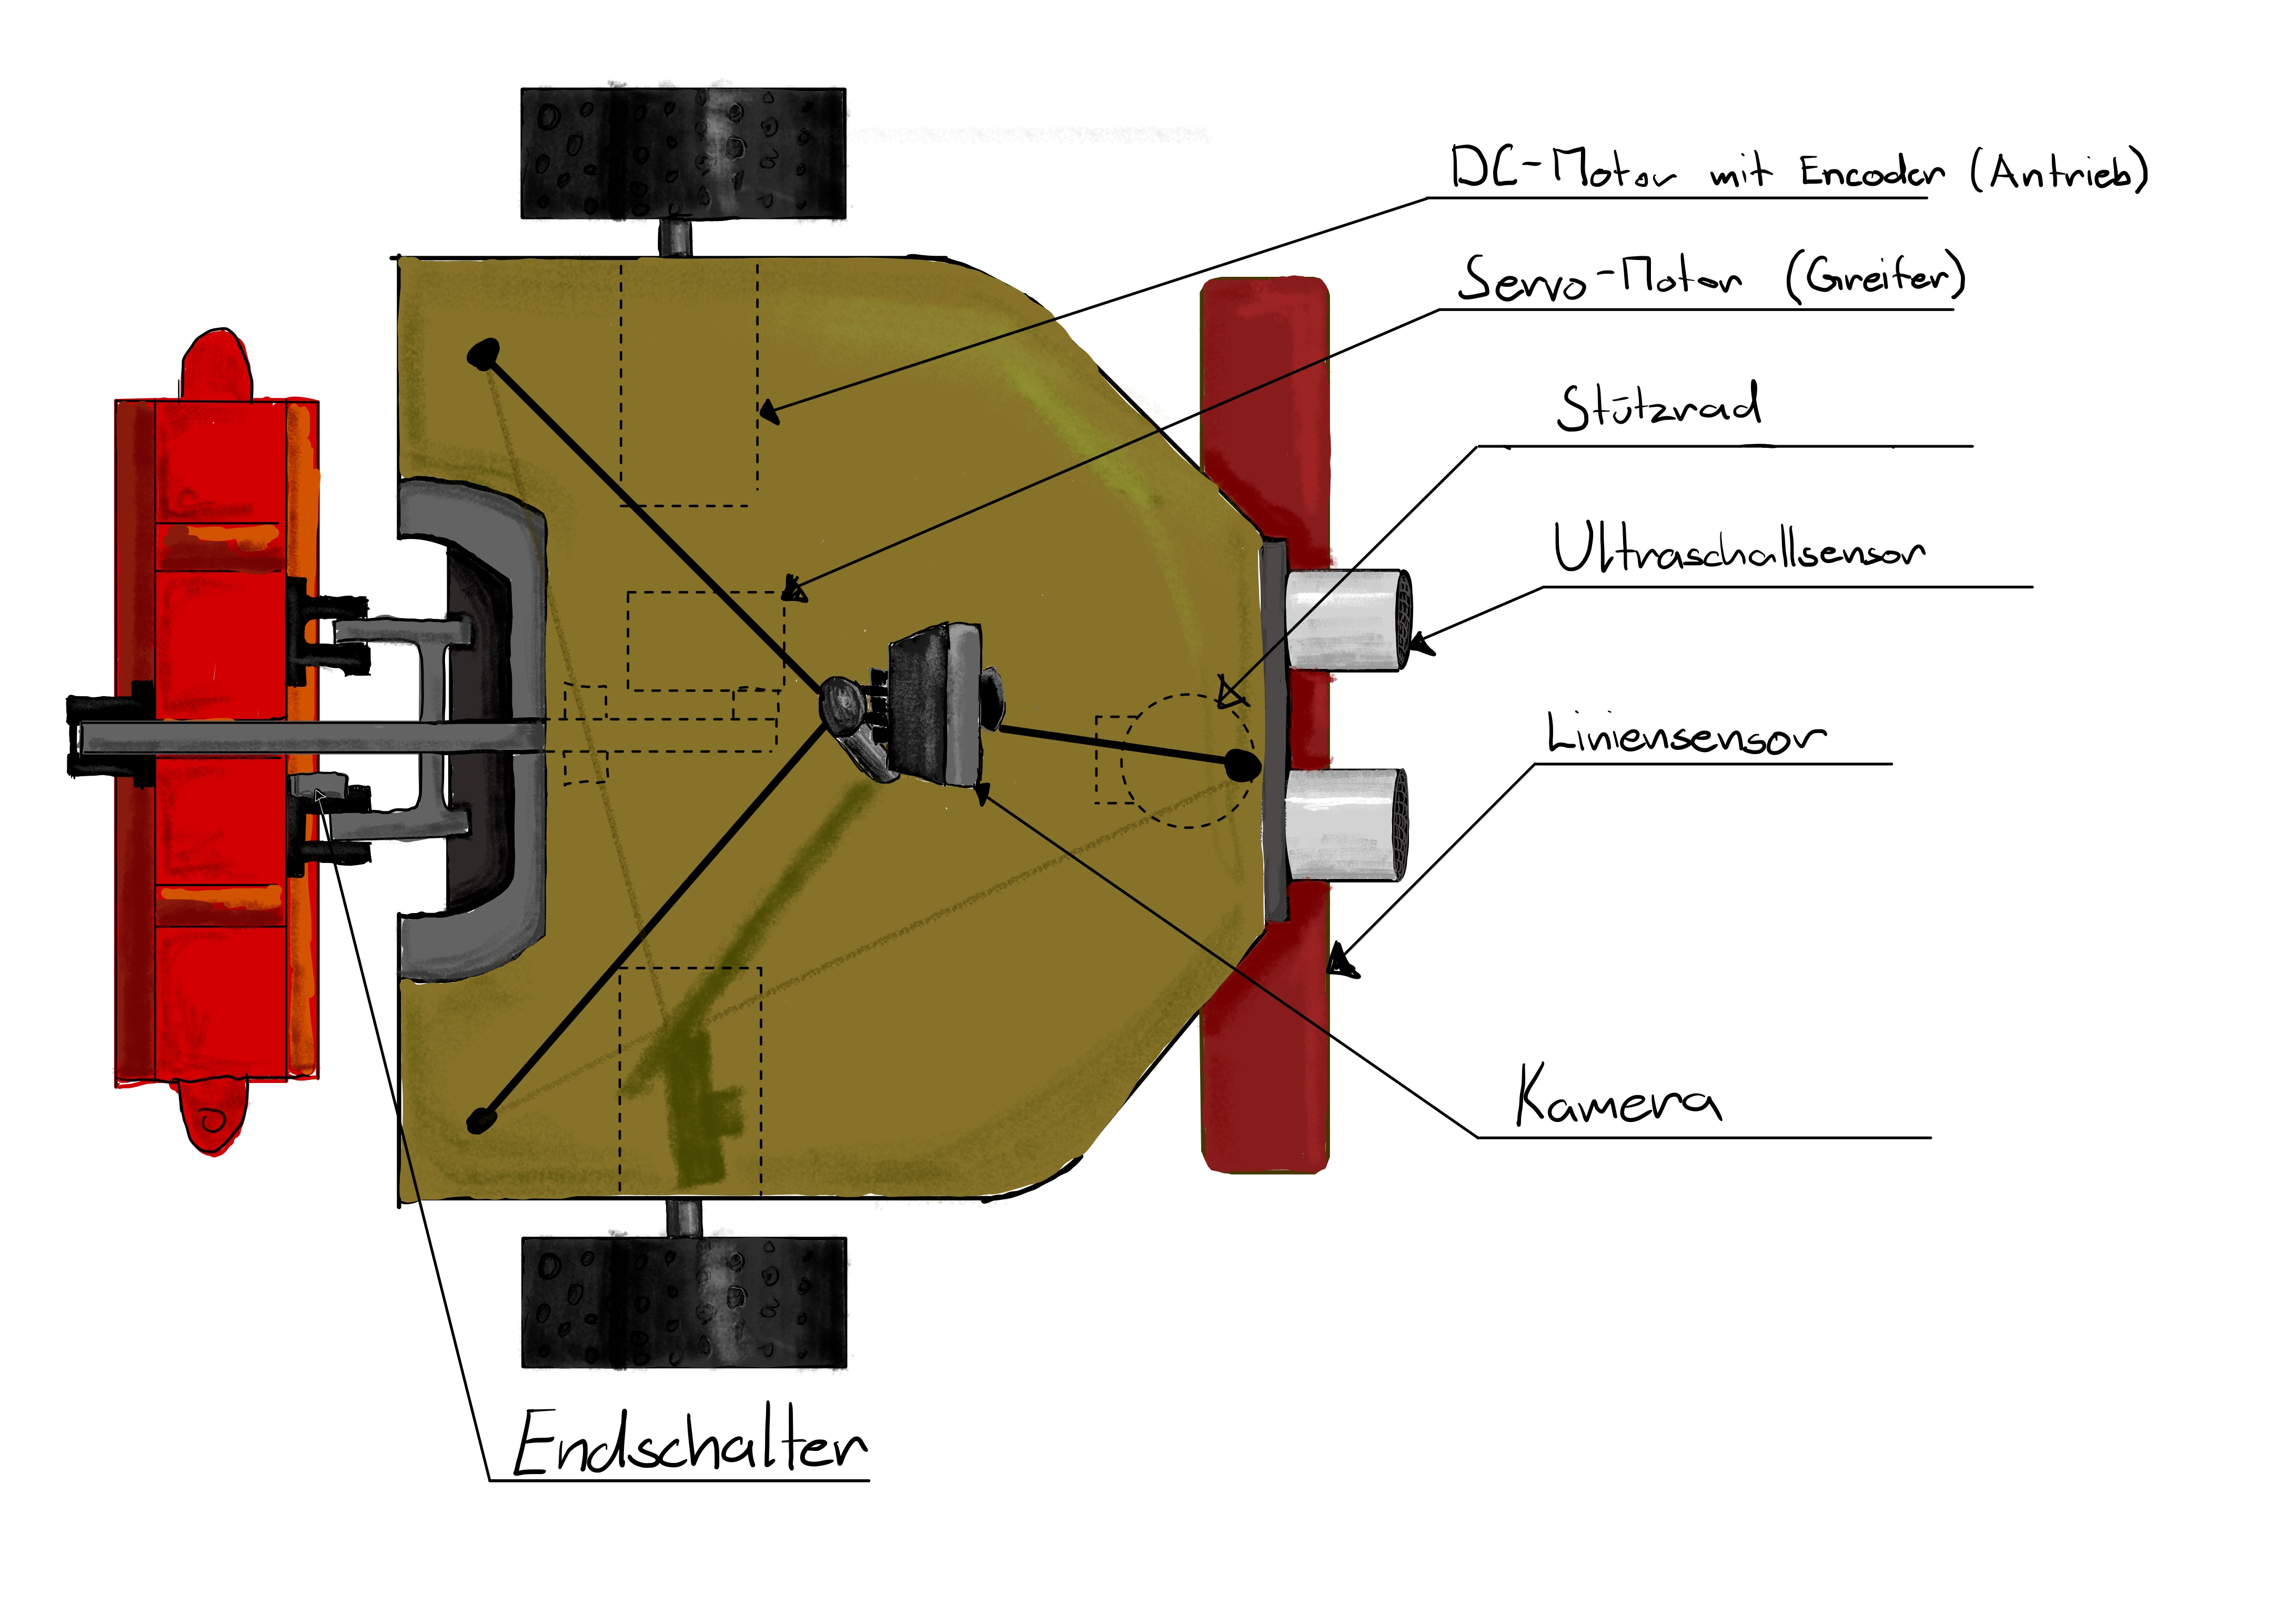
\includegraphics[width=\textwidth]{assets/gesamtkonzept/Skizze-Fahrzeugkonzept-Beschriftet.jpg}
\caption{Konzeptskizze Gesamtkonzept}
\label{fig:robot_concept-scetch_labeld}
\end{figure}


\subsection{Komponenten}

Folgendes Komponenten für das Konzept wurden mithilfe der Technologierecherche (siehe Anhang \ref{techrecherche}) und anschliessenden morphologische Kästen (siehe Anhang \ref{mk}) und Nutzwertanalysen (siehe Anhang \ref{nutzwertanalyse}) ermittelt. 

\begin{table}[H]
\centering
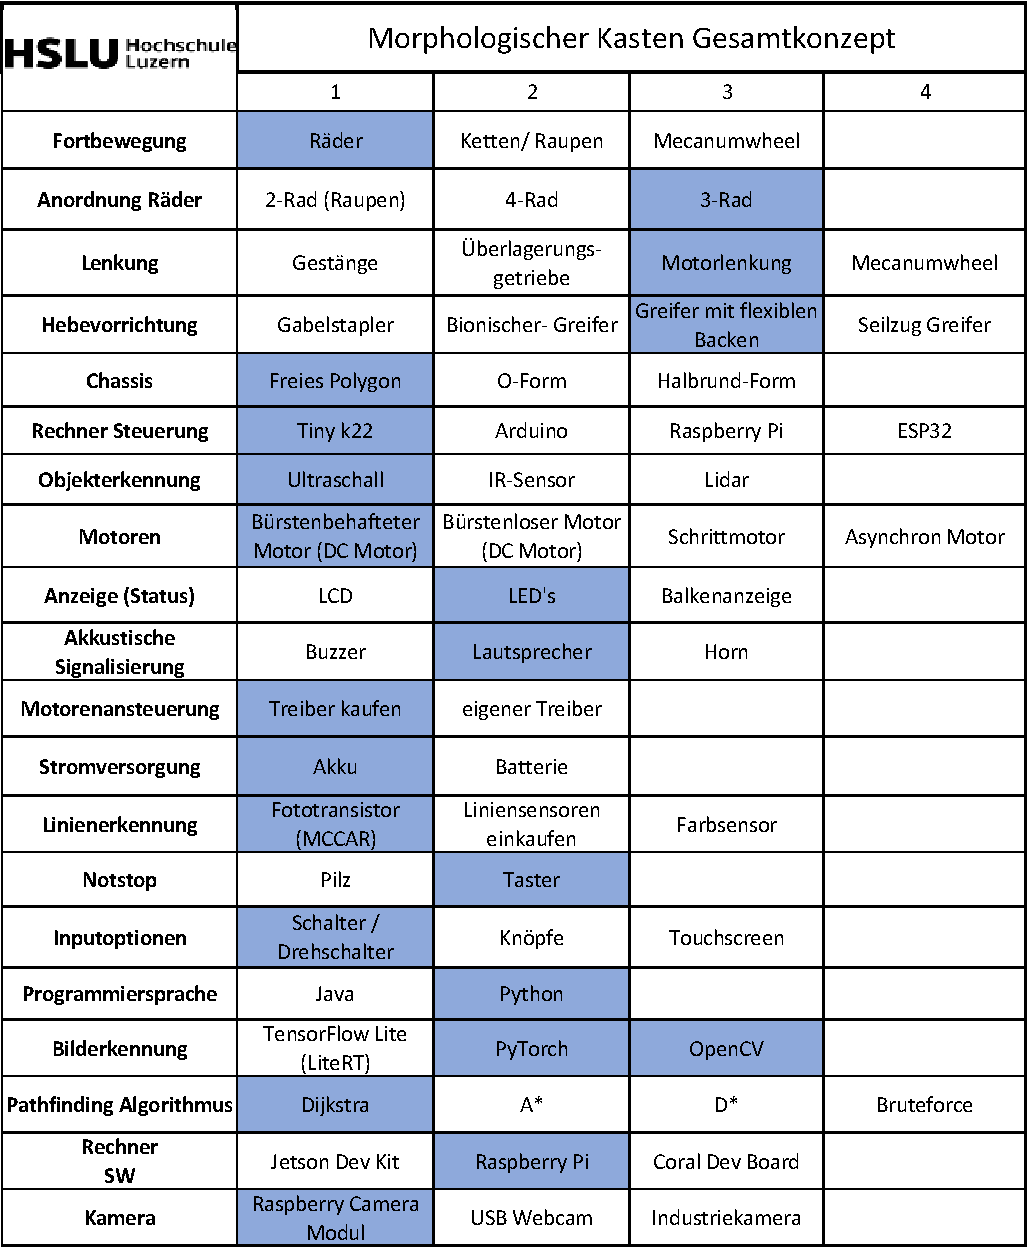
\includegraphics[width=\textwidth -20mm]{assets/MK-all.pdf}
\caption{Morphologischer Kasten: Gesamtkonzept}
\label{table:mk-all}
\end{table}

Es ist geplant einen Roboter in U-Form zu bauen, der sich mit drei Rädern fortbewegt und eine Motorlenkung besitzt. Hindernisse kann der Roboter mit einem Parallelgreifer anheben.

Die Steuerung wird auf einem Tiny k22 laufen. Die Distanz zu den Objekten wird mit Ultraschall erkannt. Die bürstenbehafteten Motoren werden mit einem gekauften Treiber angesteuert. Die Stromversorgung läuft über einen Akku. Der Akkustand und der Status des Roboters werden mit LED's angezeigt. Damit der Roboter die Linien erkennt, wird ein Liniensensor mit Fototransistoren verwendet. Das Ziel wird über einen Schalter vom Benutzer ausgewählt.
Wenn der Roboter das Ziel erreicht, verkündet er dies über einen Lautsprecher. Im Notfall wird der Roboter über einen Taster ausgeschaltet.

Die Software wird in Python geschrieben und läuft auf einem Raspberry Pi. Zur Bilderkennung wird eine Kombination von PyTorch und OpenCV verwendet. Die Bilder werden mit einer Raspberry Camera aufgenommen. Der kürzeste Weg wird mit einem Dijkstra Algorithmus berechnet.


\subsection{Ablauf}

Die Schritte, die mit einem Plus markiert sind, sind in den folgenden Kapiteln als Subprozesse detailliert definiert.

\begin{figure}[H]
\centering
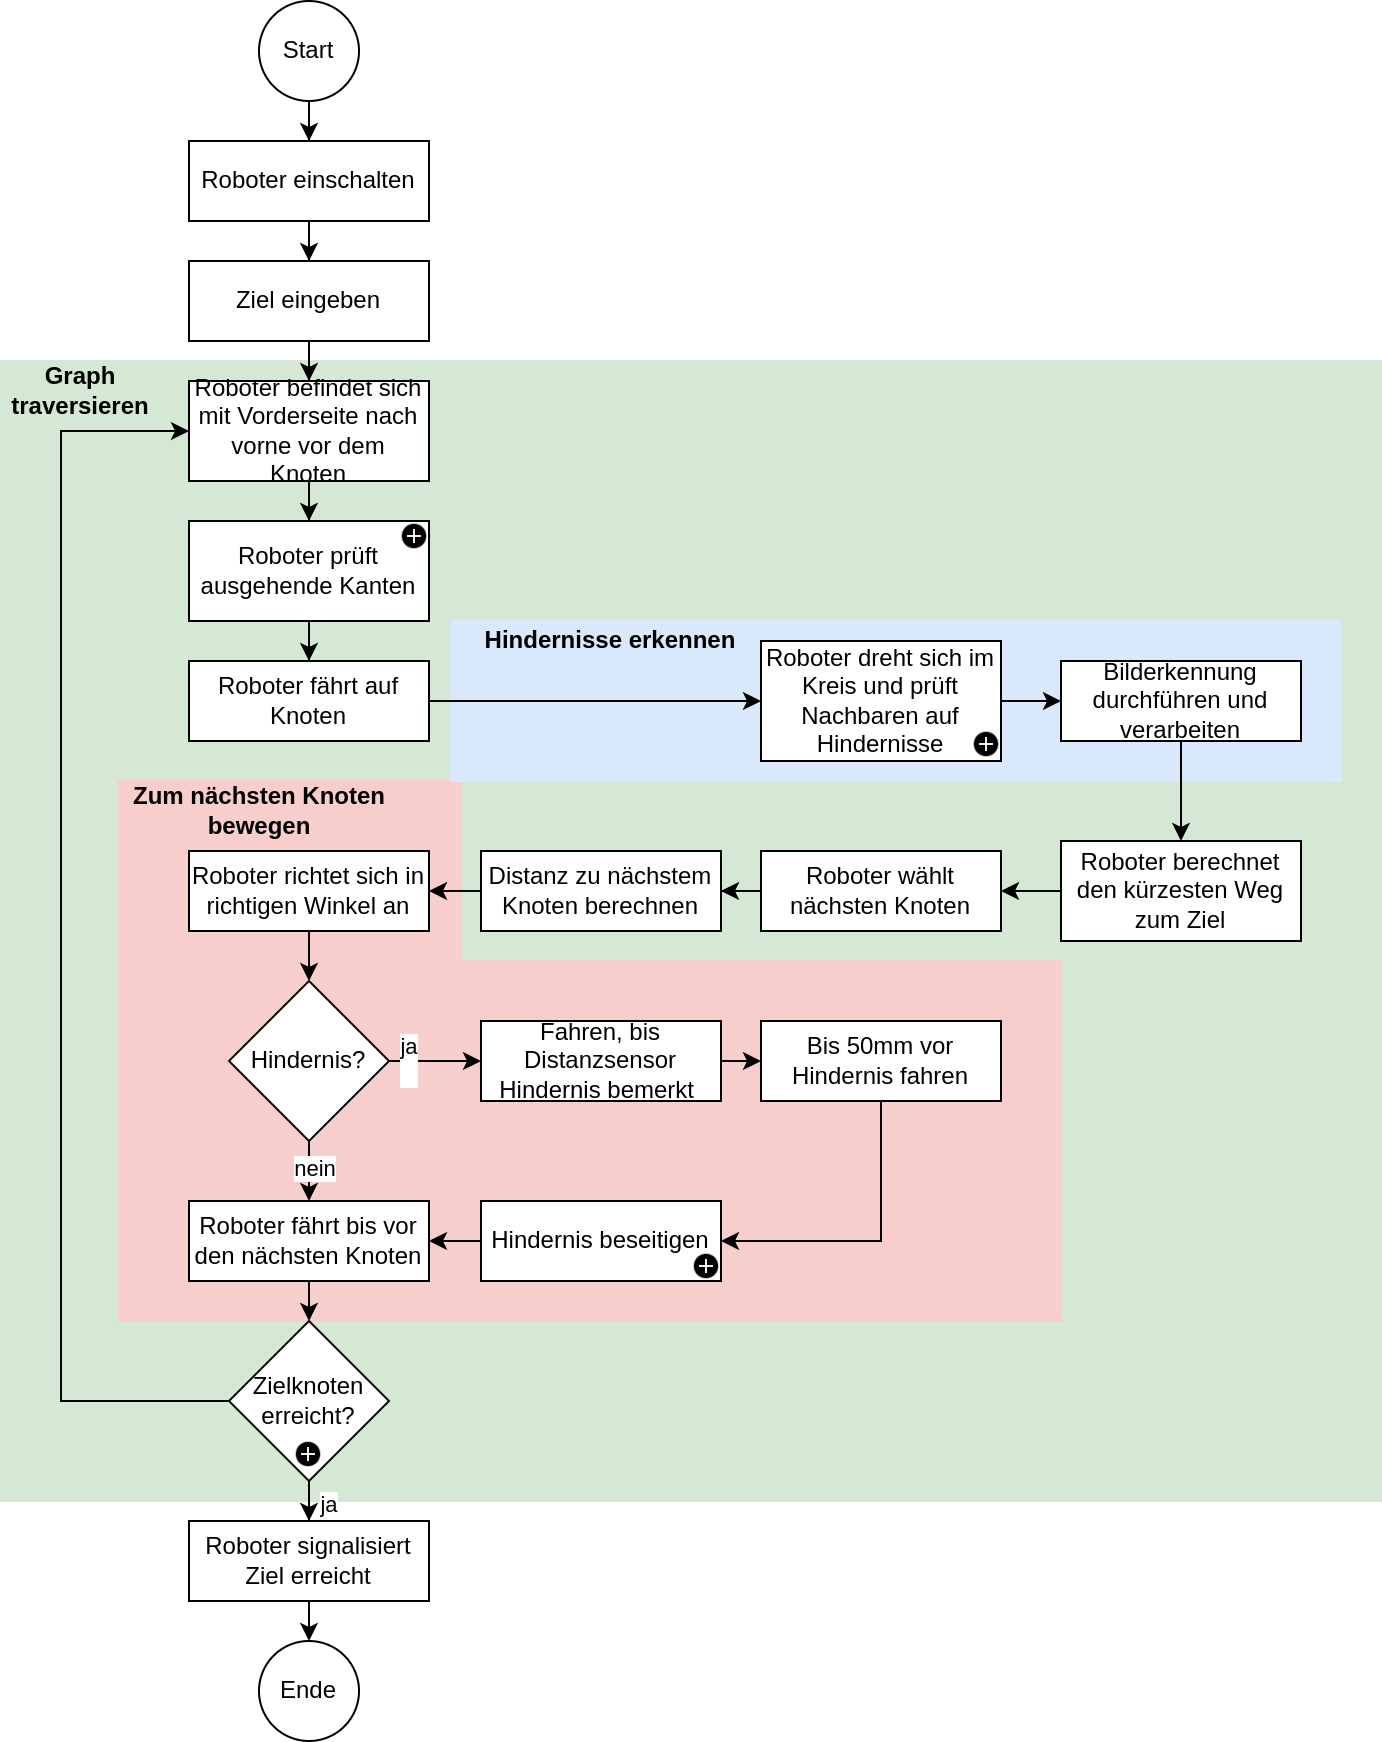
\includegraphics[width=\textwidth]{assets/gesamtkonzept/ablaufdiagramm.png}
\caption{Ablaufdiagramm}
\label{fig:ablaufdiagramm}
\end{figure}

\subsubsection{Fortbewegung}

PLACEHOLDER

\subsubsection{Linienerkennung}

PLACEHOLDER

\subsubsection{Wegfindung}

Der kürzeste Weg im Graphen vom momentanen Knoten zum Zielknoten wird mit dem Dijkstra Algorithmus\footnote{https://www.w3schools.com/dsa/dsa\_algo\_graphs\_dijkstra.php} berechnet. Diese wird zum Beginn berechnet und jedes Mal, wenn der Roboter neue Erkenntnisse zum Graph gesammelt hat, welche die Zielführung beeinflussen kann.

Zusätzlich zum zukünftigen Pfad, wird auch der bereits befahrene Pfad gespeichert. Dies dient dazu, dass der Roboter immer in der Lage sein wird im Fehlerzustand, auf den letzten Knoten zurückzufahren und immer noch weiss, wo er sich befindet.

\subsubsection{Kameraposition}

Die Kamera wird in einer Höhe von 22.5cm und einem Winkel von 56\textdegree\ montiert. Die Position dieser ist fix, das heisst wir benötigen keine schwenkbare Kamera.
Die Kamera selbst verfügt über ein Horizontales Field of View\footnote{\url{https://en.wikipedia.org/wiki/Field_of_view}} von 66\textdegree. Wir verwenden die Kamera im Hochformat, Somit haben wir im Field of View von 66\textdegree\ sowohl sehr nahe Knoten und Objekte bis zu 10cm im Bild. Aber auch weit entfernte Pylonen, welche 200cm entfernt stehen.

\begin{figure}[H]
    \centering
    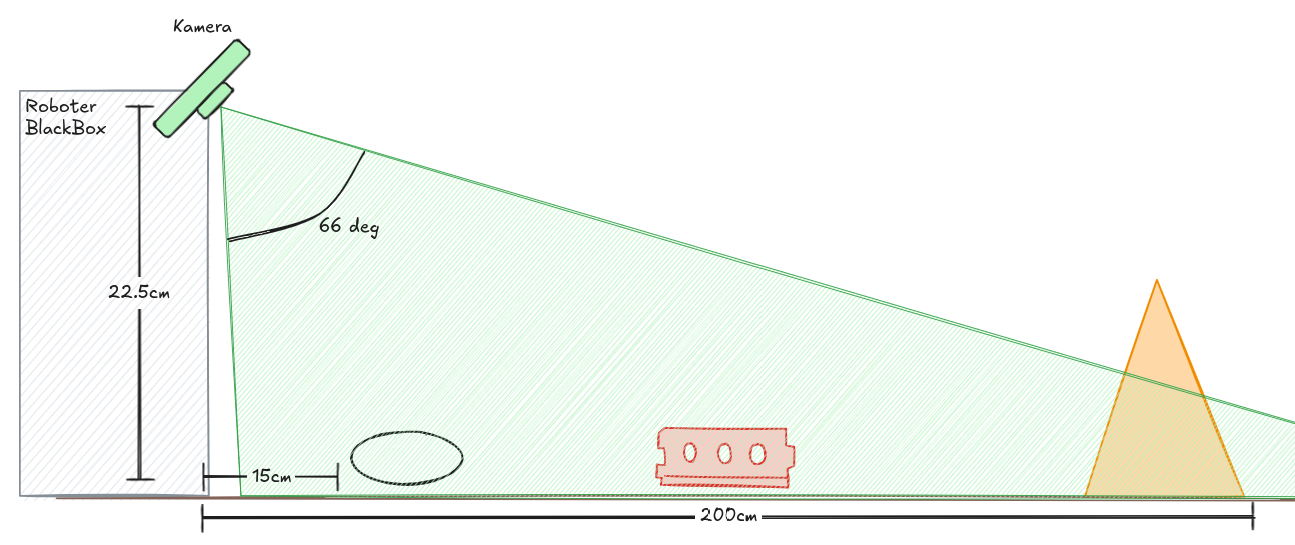
\includegraphics[width=1\linewidth]{assets//informatik-prototyp//camera/camera_position.png}
    \caption{Kamera Positionierung}
    \label{fig:camera-position-concept}
\end{figure}

\subsubsection{Ausgehende Kanten erkennen}

\begin{figure}[H]
\centering
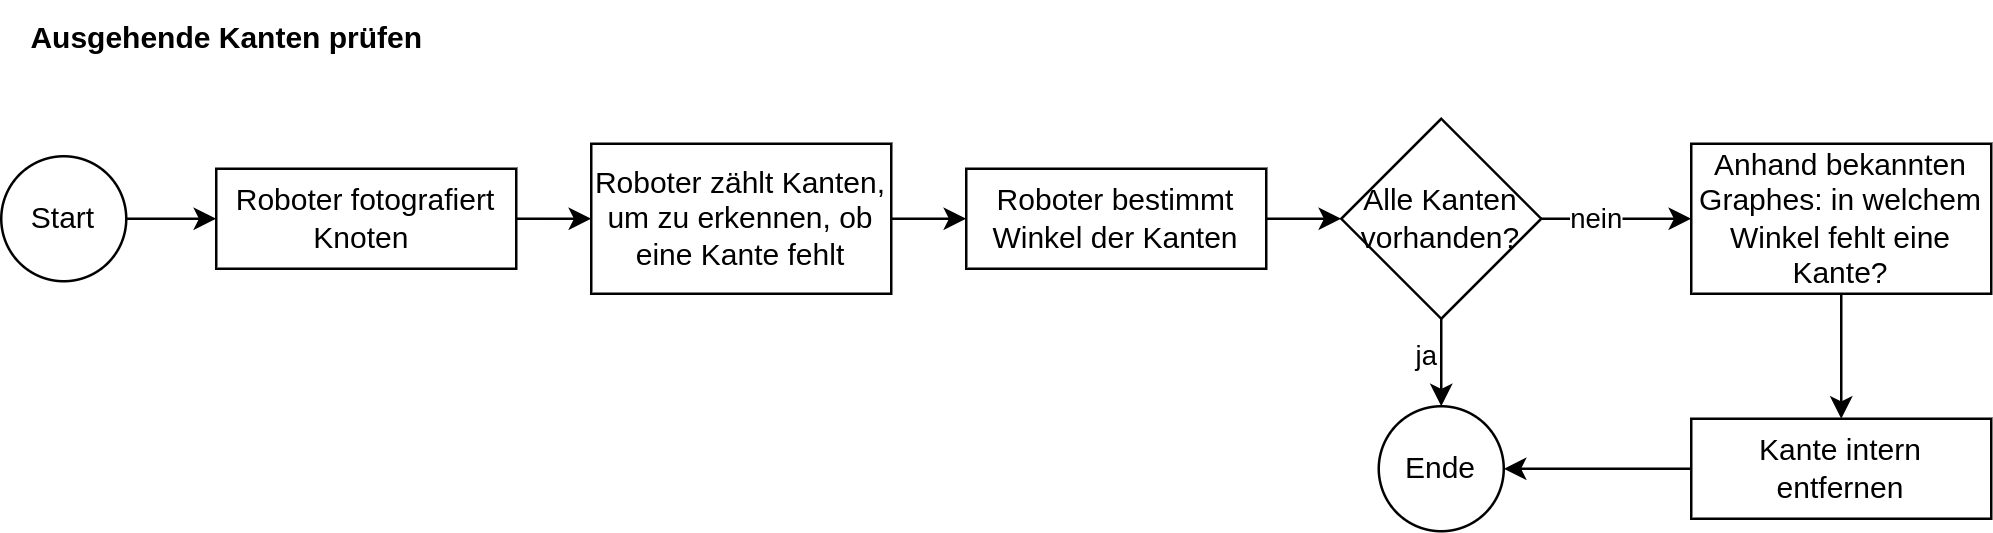
\includegraphics[width=\textwidth]{assets/gesamtkonzept/ablaufdiagramm-kanten-erkennen.png}
\caption{Ablaufdiagramm ausgehende Kanten erkennen}
\label{fig:ablaufdiagramm-kanten-erkennen}
\end{figure}

Der Roboter bewegt sich auf einen Knoten zu und hält 15 cm vor diesem an. Der Knoten wird fotografiert und der Roboter fährt anschliessend auf den Knoten. Das Bild wird rotiertet und mit OpenCV zuerst so verzerrt, sodass der Knoten gerade von oben dargestellt wird. Danach werden die einzelnen Winkel gemessen. Dies ist im Prototyping Kapitel im Anhang \ref{winkelerkennung} ausführlicher beschrieben. Das Resultat dieser Objekterkennung ist eine Liste mit Winkeln.

\begin{figure}[H]
\begin{subfigure}{0.55\textwidth}
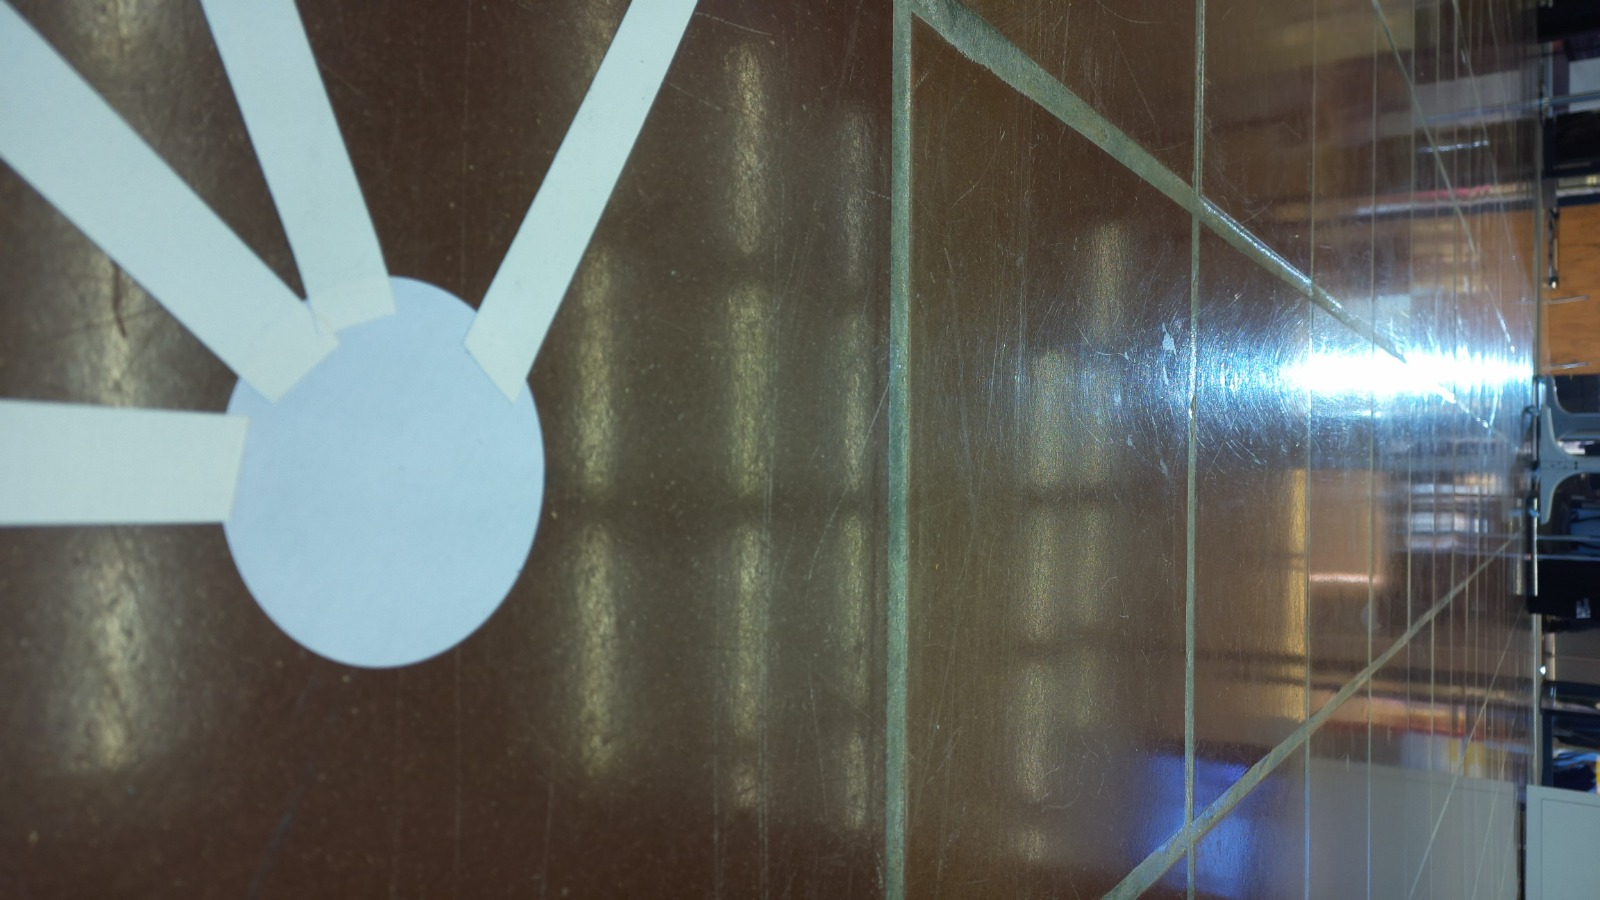
\includegraphics[width=0.95\linewidth]{assets/informatik-prototyp/opencv/knoten-bild.jpeg} 
\caption{Knoten mit 15cm Abstand}
\label{fig:node-15cm-before}
\end{subfigure}
\begin{subfigure}{0.4\textwidth}
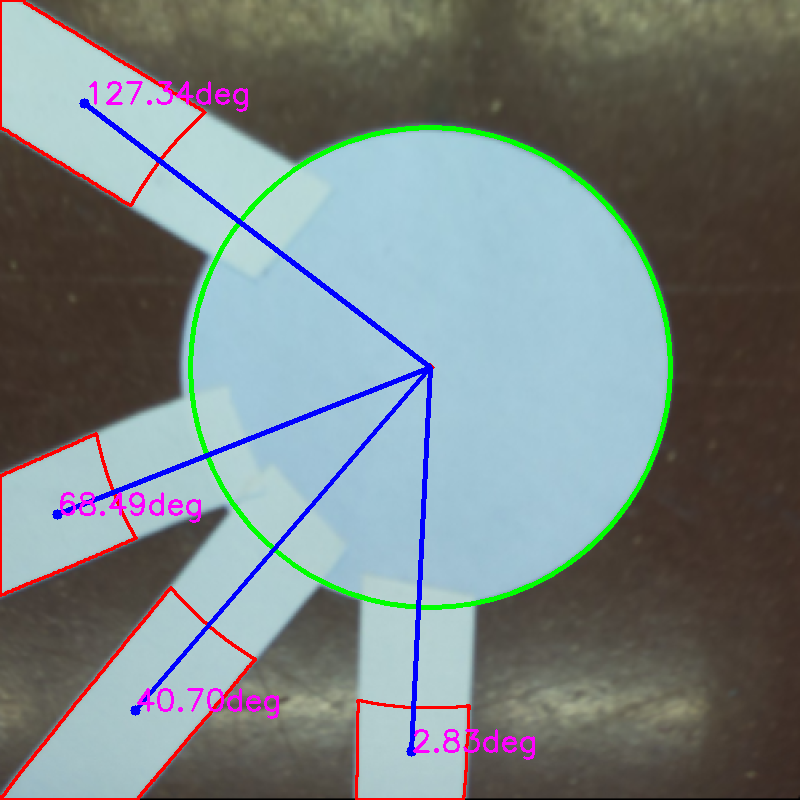
\includegraphics[width=0.95\linewidth]{assets/informatik-prototyp/opencv/angle_detection/node_with_edge_angles_annotated.png} 
\caption{Knoten mit gemessenen Winkeln}
\label{fig:node-angles}
\end{subfigure}

\caption{Winkelerkennung}
\label{fig:angle-recognition}
\end{figure}

Die erhaltene Liste mit Winkeln wird nun verwendet, um mögliche fehlende Linien zu erkennen und die Winkel intern zu speichern. Die internen Winkel werden verwendet, um den Roboter richtig auszurichten, wenn dieser auf die nächste Linie fährt.

Der Roboter selber hat einen Grundgraphen mit Winkeln gespeichert. Diese Winkel ergeben sich aus dem zur Verfügung gestellten Graph.
Da der Graph nicht genau so aufgeklebt sein wird, wie auf der Skizze, wurden Bereiche definiert, in denen sich die Winkel befinden sollten.

Ein Ausschnitt, der zeigt, wie der interne Graph in einem YAML File definiert ist, ist hier eingefügt.

\begin{verbatim}
C: [{D: [60, [30, 120]}, {B: [240, [120, 30]}, {H: [60, [30, 30]}]
\end{verbatim}

Auf Grafik a) sind alle Winkel eingezeichnet inklusive der Halbwinkel zwischen allen Kanten. In Grafik b) ist die Kante zwischen C und D gezeigt, dies entspricht \verb|'C: [{D: [60, [30, 120]}'| im YAML File. Wenn der Roboter sich von Knoten C zu Knoten D bewegen möchte, dann wäre diese Kante im Idealfall 60\textdegree\ von der Kante links aus. Das der Idealfall nicht eintreten wird, sind die Halbwinkel eingezeichnet, hier 30\textdegree\ und 120\textdegree. Von der linksliegenden Kante aus, darf kann sich die Kante zu Knoten D also im Bereich von 60\textdegree-30\textdegree\ und 60\textdegree+120\textdegree, sprich 30\textdegree\ und 180\textdegree\ befinden. Befindet sich eine gemessene Kante in diesem Bereich, wird es die Kante C zu D sein.

\begin{figure}[H]
\begin{subfigure}{0.62\textwidth}
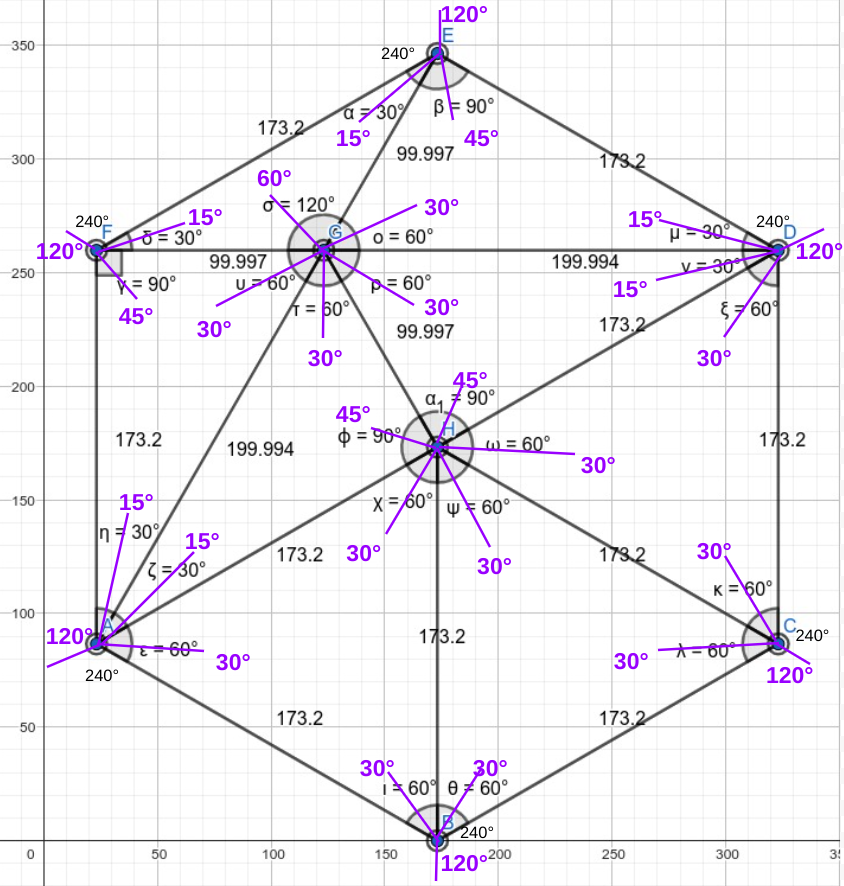
\includegraphics[width=0.95\linewidth]{assets/informatik-prototyp/graph-angles.png} 
\caption{Graph mit Winkeln und Winkelbereichen}
\label{fig:angled-graph}
\end{subfigure}
\begin{subfigure}{0.38\textwidth}
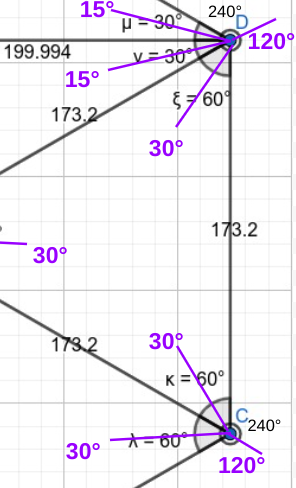
\includegraphics[width=0.95\linewidth]{assets/informatik-prototyp/c-d-angle.png} 
\caption{C zu D Winkel}
\label{fig:excerpt-angled-graph}
\end{subfigure}
\caption{Winkel im Graphen}
\label{fig:angles}
\end{figure}

Als erstes wird die Länge der Liste mit Winkeln gemessen. Wenn sich gleich viele Winkel darin befinden, wie es laut dem Grundgraphen ausgehende Linie haben soll, dann bedeutet das, dass keine Linie fehlt. In diesem Fall werden die internen Winkel aktualisiert mit den tatsächlichen Werten. 

Falls es weniger Winkel gibt als erwartet, werden die erhaltenen Winkel zu den einzelnen möglichen Bereichen zugeordnet. In diesem Bereich, dem kein Winkel zugeordnet wurde, fehlt eine Linie. Folglich aktualisiert der Roboter seine internen Informationen: eine Linie wird aus dem Grundgraphen entfernt und die anderen Winkel werden mit den gemessenen Werten ersetzt.

Nachdem der Roboter den nächsten Knoten berechnet hat, wird der Winkel zur richtigen ausgehenden Kante an die Steuerung gesendet. Der Roboter dreht sich, um auf dieser Linie weiterzufahren.

\subsubsection{Zielknoten erkennen}

PLACEHOLDER OpenCV OpenCV right? Still in prototyping stage... Not yet documented.


\subsubsection{Pylonen und Hindernisse erkennen}

\begin{figure}[H]
\begin{subfigure}{0.45\textwidth}
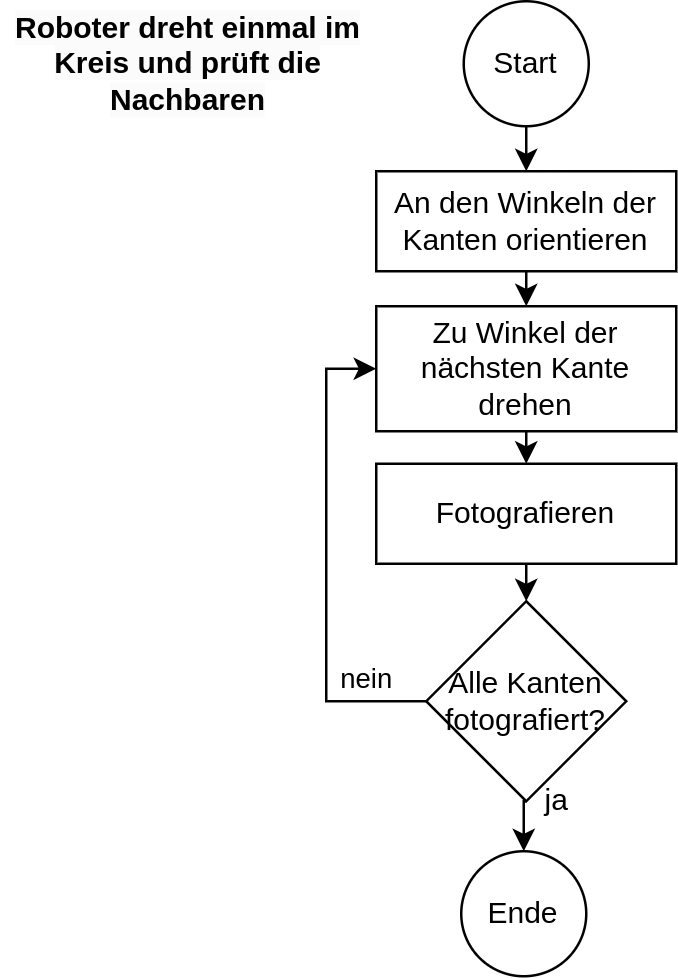
\includegraphics[width=\textwidth]{assets/gesamtkonzept/ablaufdiagramm-hindernisse-erkennen.png}
\caption{Ablaufdiagramm Hindernis erkennen}
\label{fig:ablaufdiagramm-hindernis-erkennen}
\end{subfigure}
\begin{subfigure}{0.55\textwidth}
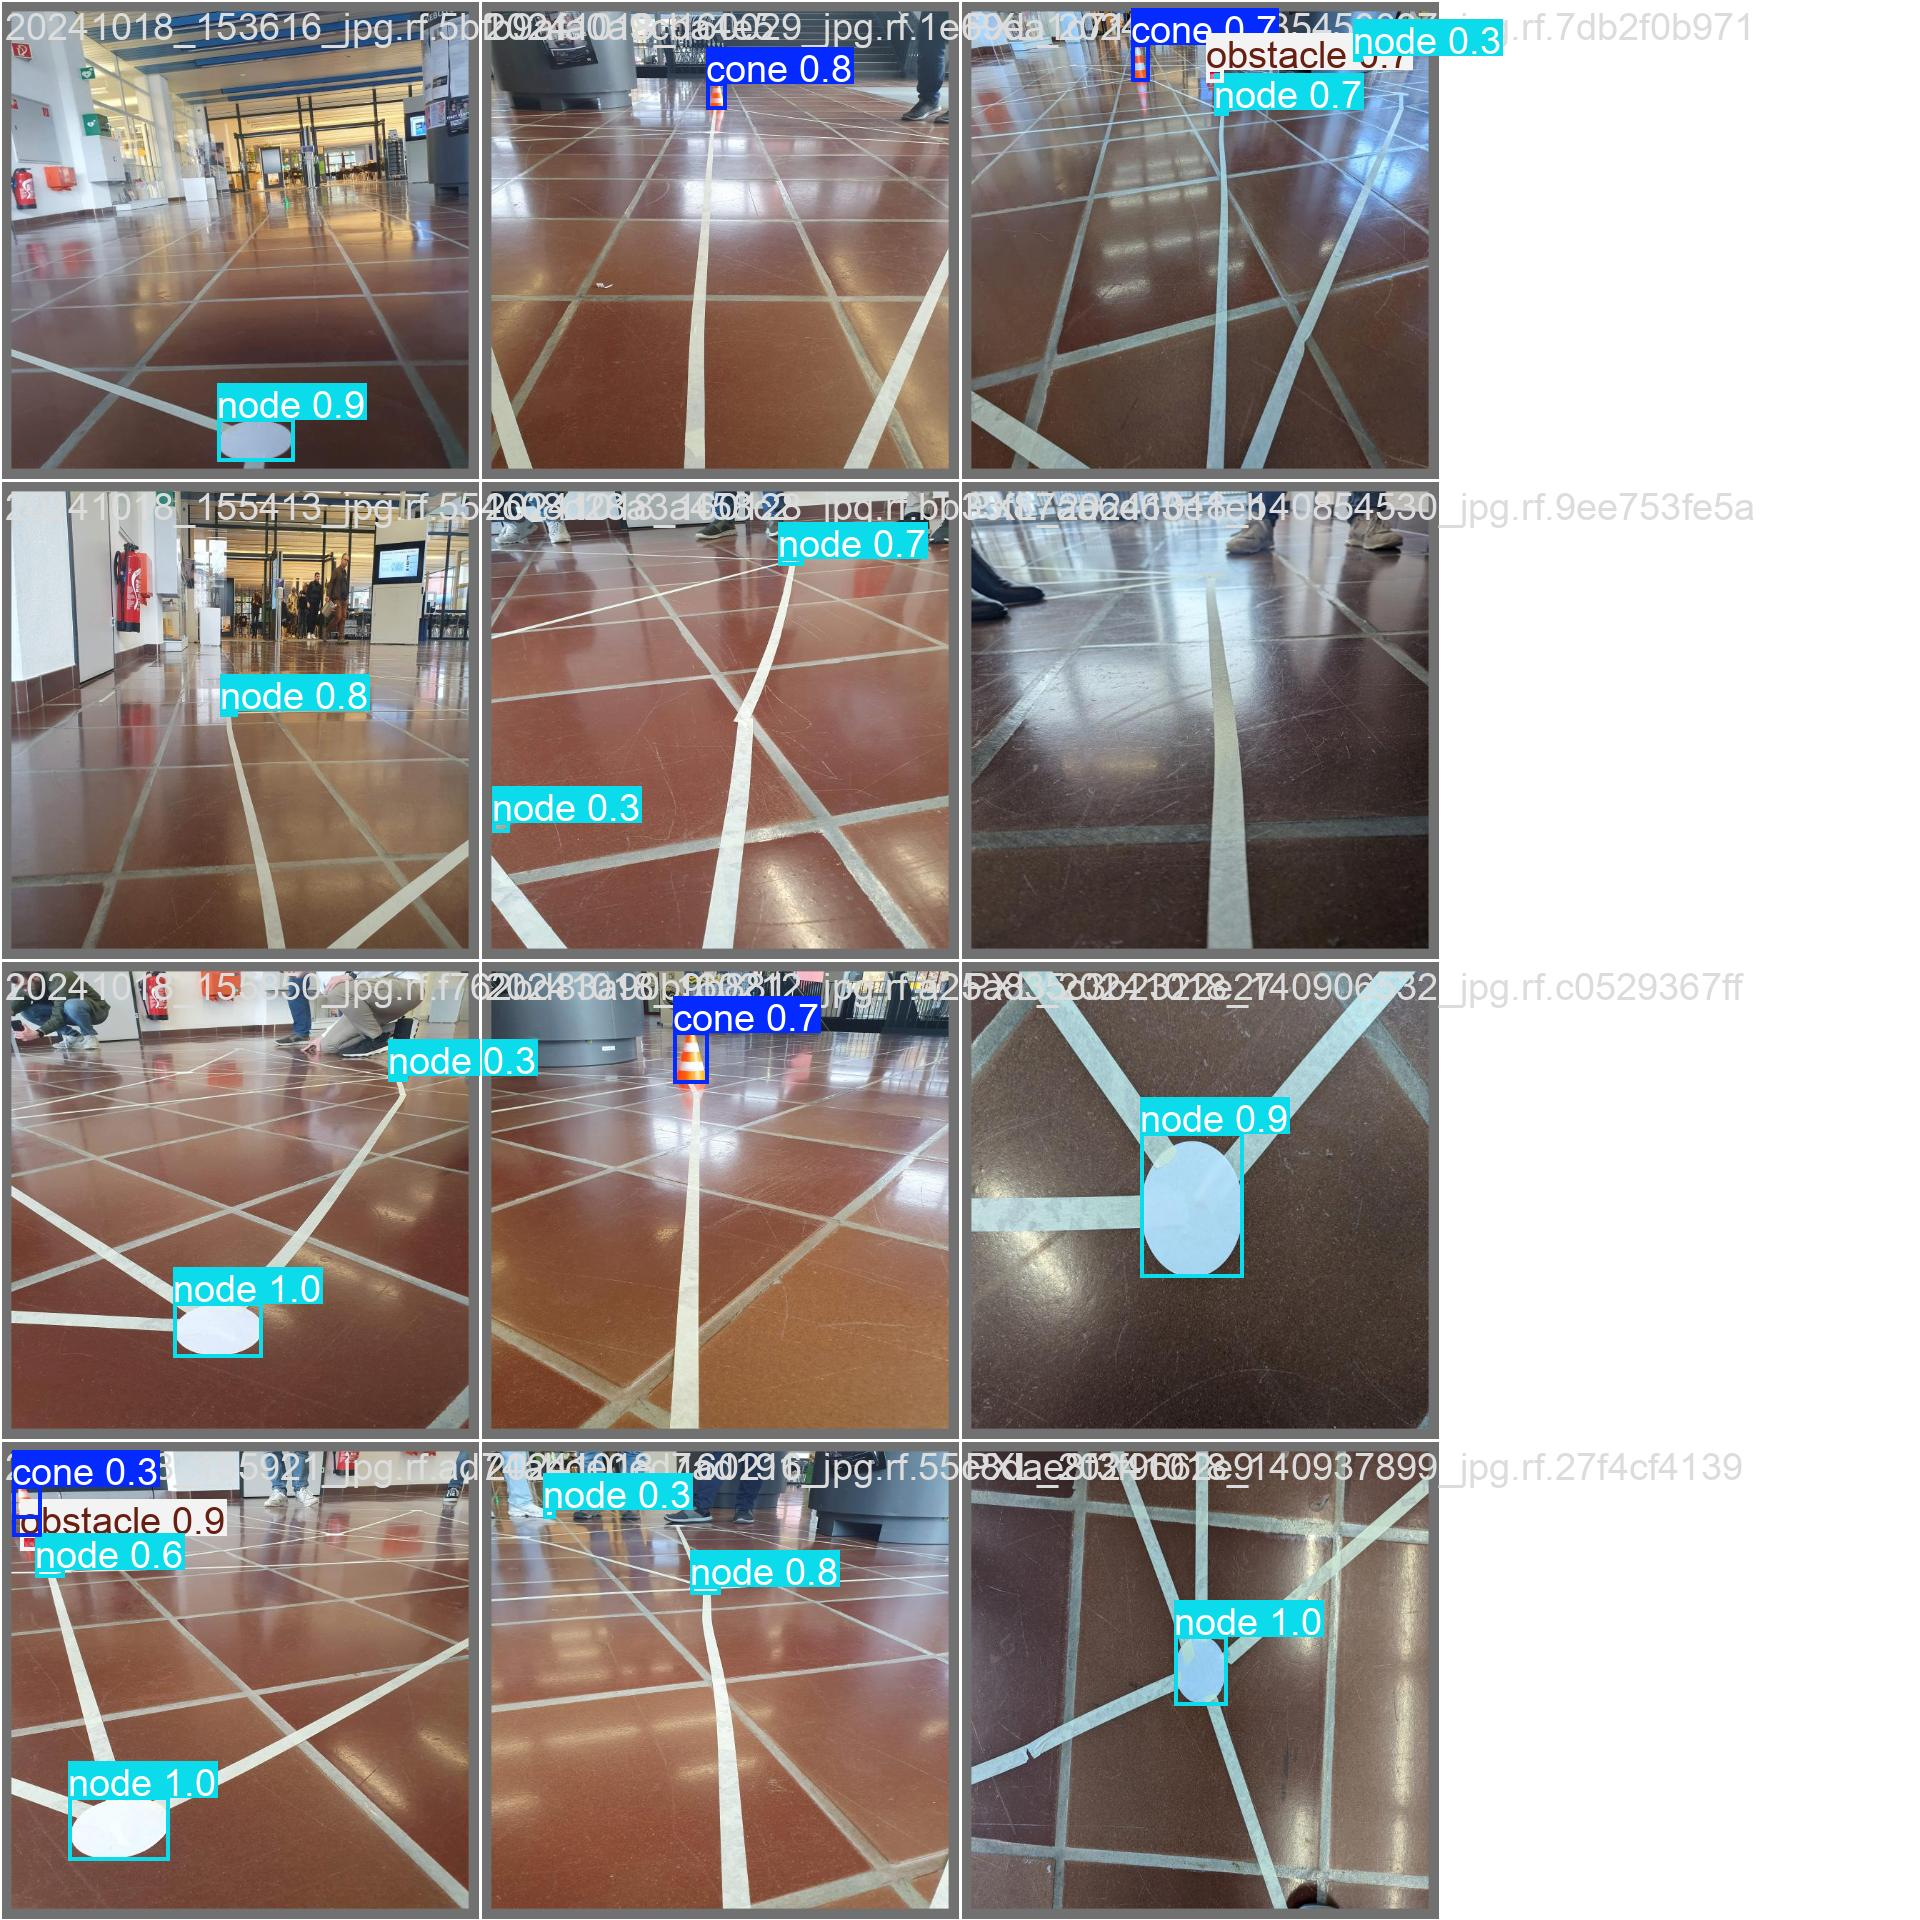
\includegraphics[width=\textwidth]{assets/informatik-prototyp/yolo/recognized-images.jpeg}
\caption{YOLOv11 Bilderkennung}
\label{fig:img-recognition-yolo}
\end{subfigure}
\caption{Bilderkennung Hindernisse}
\label{fig:image-detection-obstacles}
\end{figure}


% \begin{figure}[H]
% \centering
% 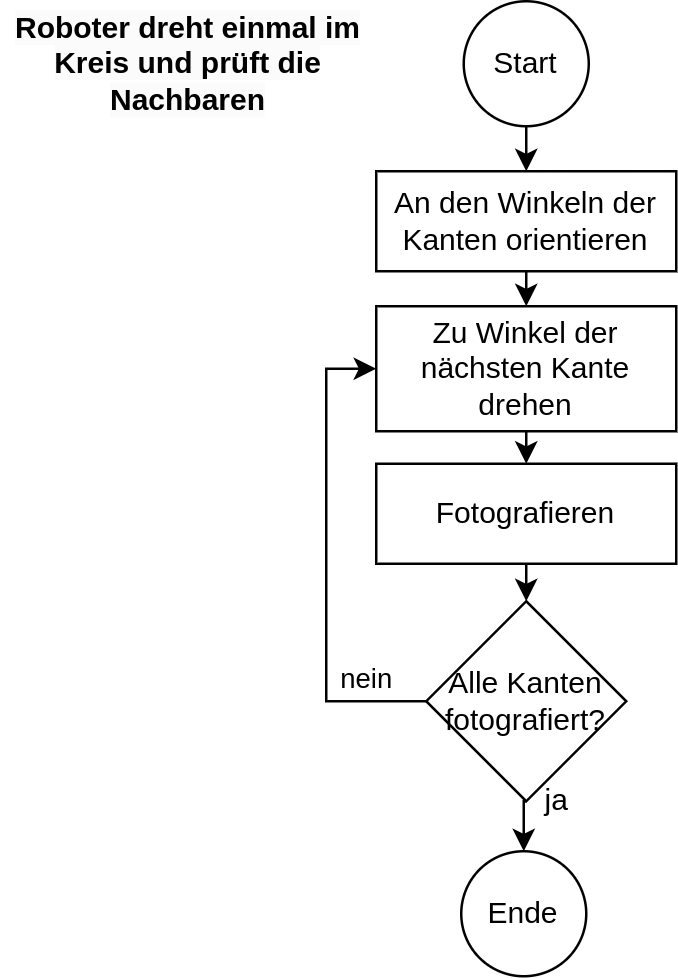
\includegraphics[width=0.35\textwidth]{assets/gesamtkonzept/ablaufdiagramm-hindernisse-erkennen.png}
% \caption{Ablaufdiagramm Hindernis erkennen}
% \label{fig:ablaufdiagramm-hindernis-erkennen}
% \end{figure}

Aus dem vorherigen Schritt der Kanten erkennen, kennt der Roboter alle ausgehenden Linien und deren Position. Er dreht sich nun im Uhrzeigersinn zu jeder Kante und fotografiert diese. Durch das Hochformat der Kameras, sieht er weit und kann auch nur die wichtigen Elemente sehen, sprich, diese, die sich auf der Linie befinden.

Die Bilder werden mit einem YOLO Objekterkennungsalgorithmus ausgewertet. Dabei werden sowohl Knoten, als auch Pylonen und Barrieren erkannt. Hindernisse werden intern gespeichert und bei der Berechnung des Weges berücksichtigt.

% \begin{figure}[H]
% \centering
% 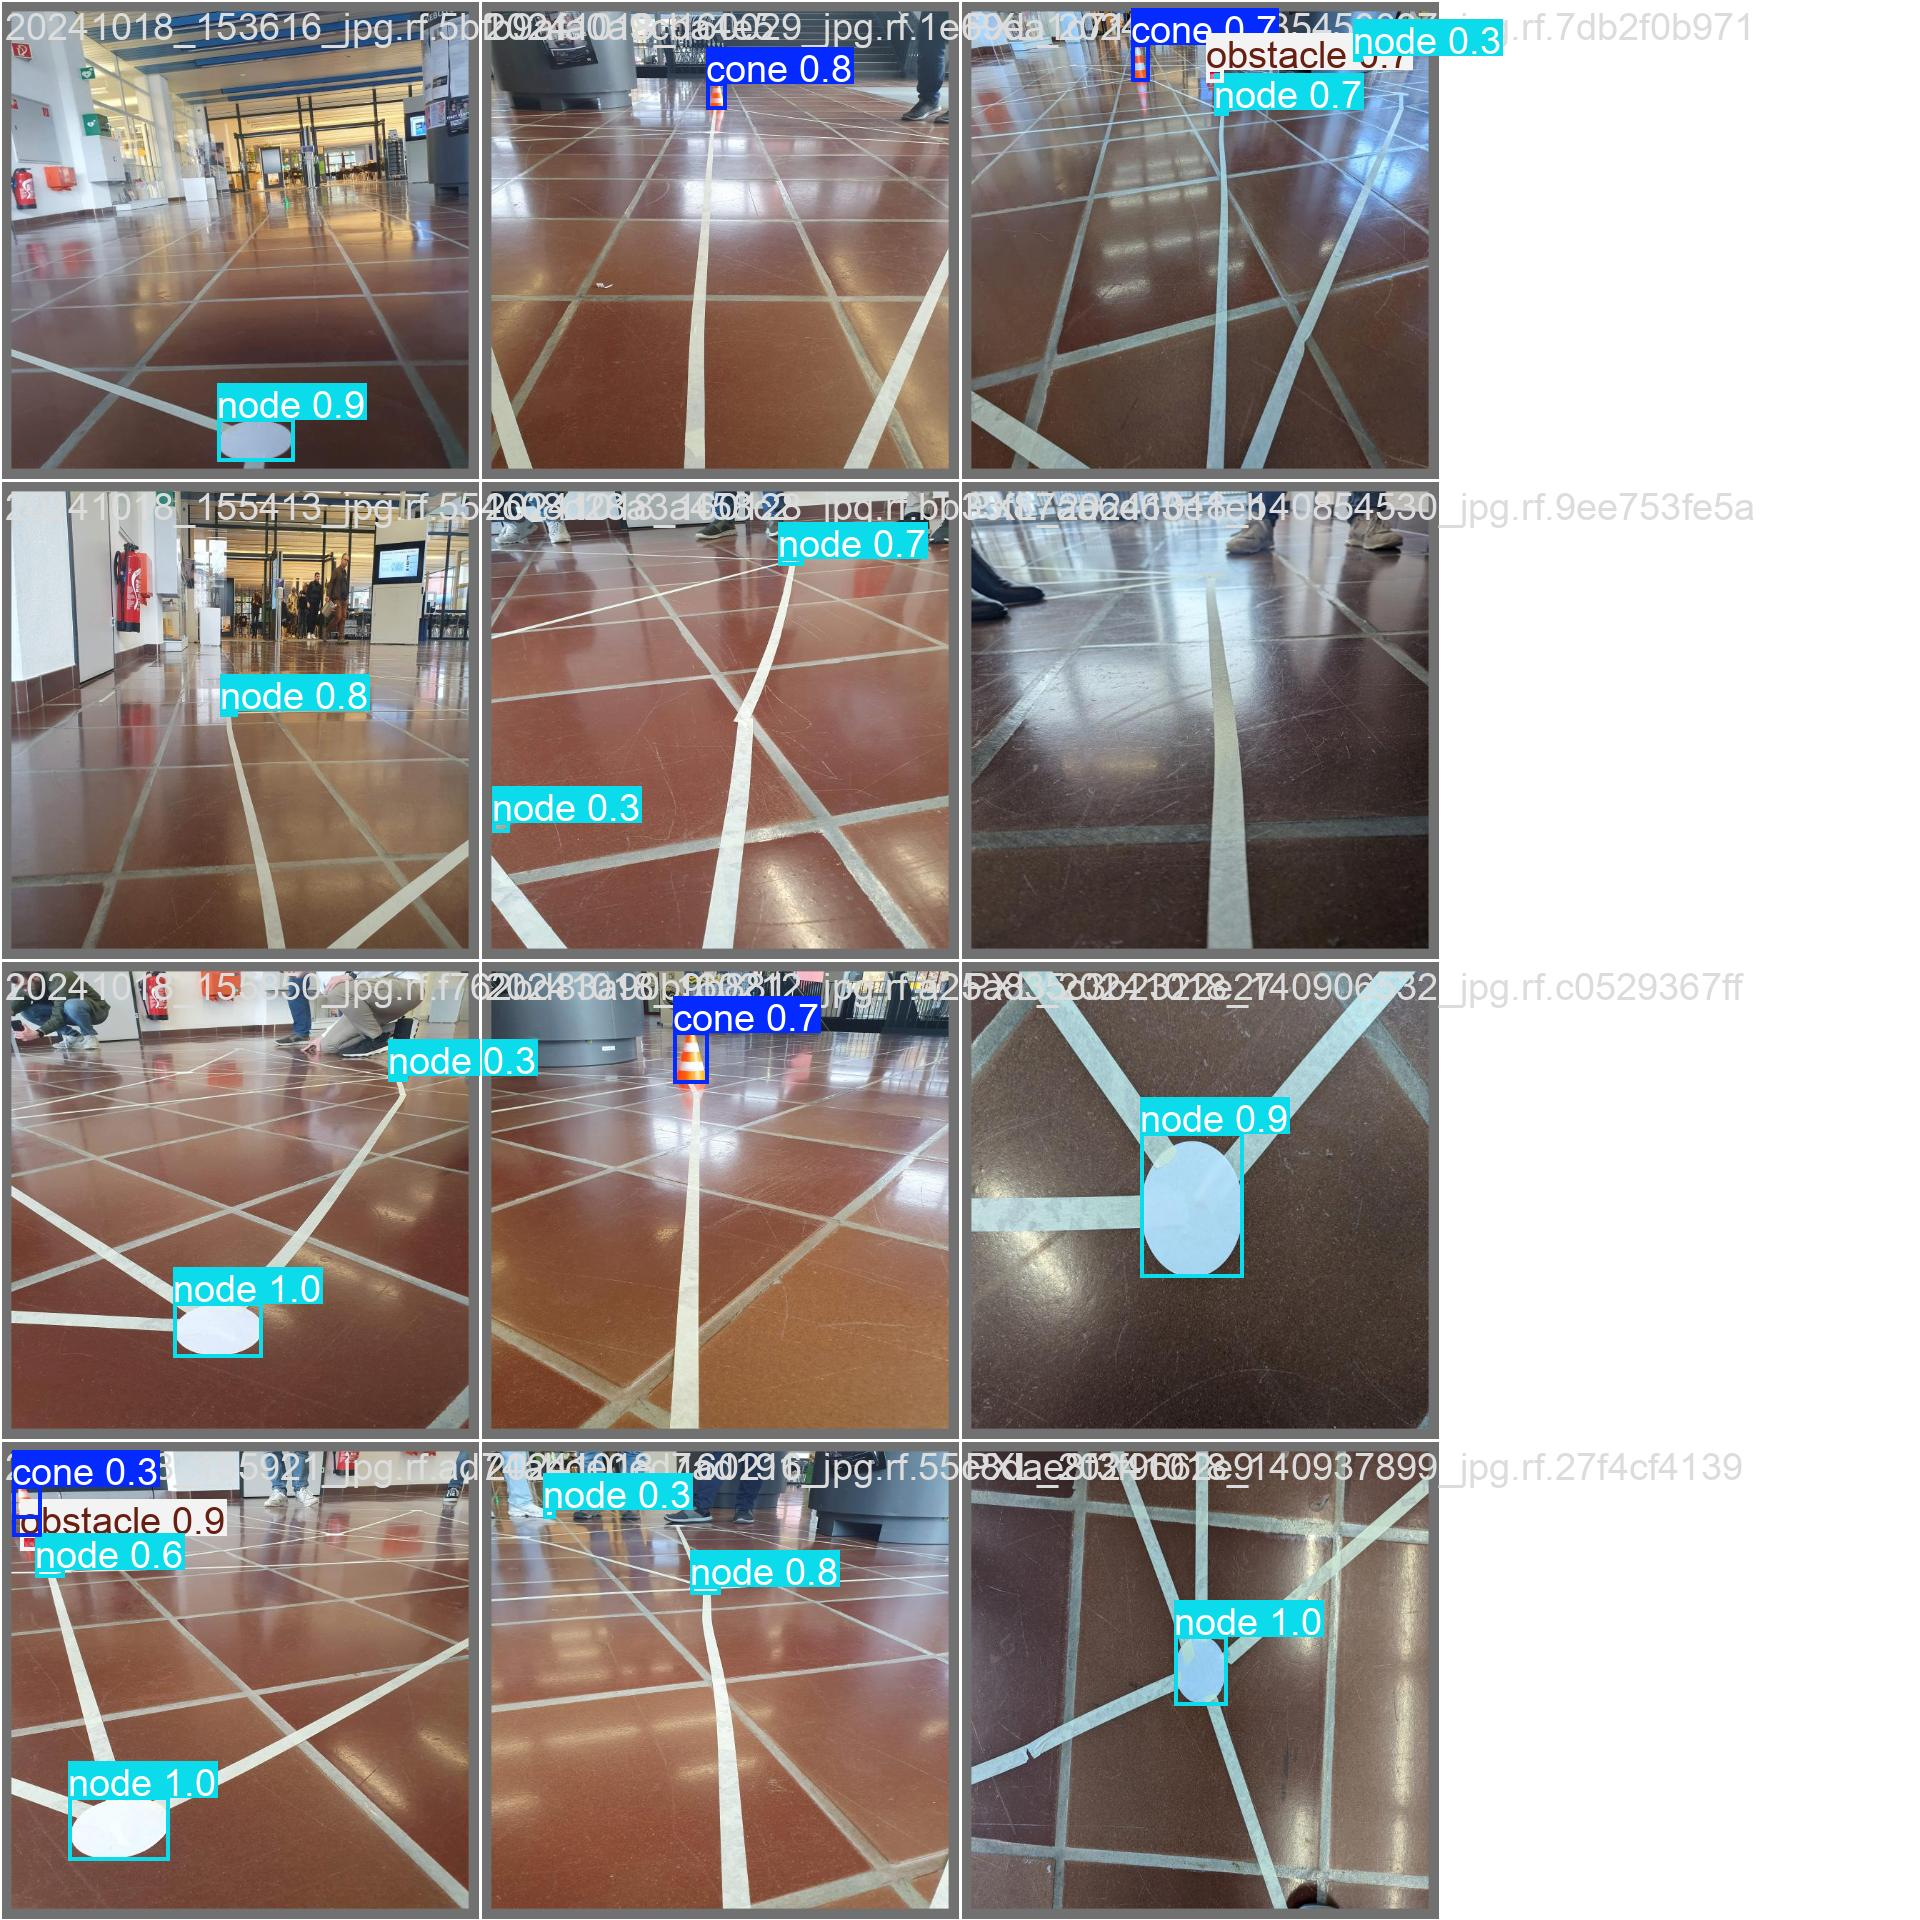
\includegraphics[width=\textwidth -30mm]{assets/informatik-prototyp/yolo/recognized-images.jpeg}
% \caption{YOLOv11 Bilderkennung}
% \label{fig:img-recognition-yolo}
% \end{figure}

\newpage

\subsubsection{Hindernisse bewegen}

In der Nutzwertanalyse (Anhang \ref{nutzwertanalyse}) hat man sich zum Anheben des Hindernisses für ein Klemm-Design entschieden, welches das Hindernis oben an der längsten Kante an 3 Punkten einspannt (siehe Abb.\ref{fig:obstacle_clamping_concept}). 

\begin{figure}[H]
\centering
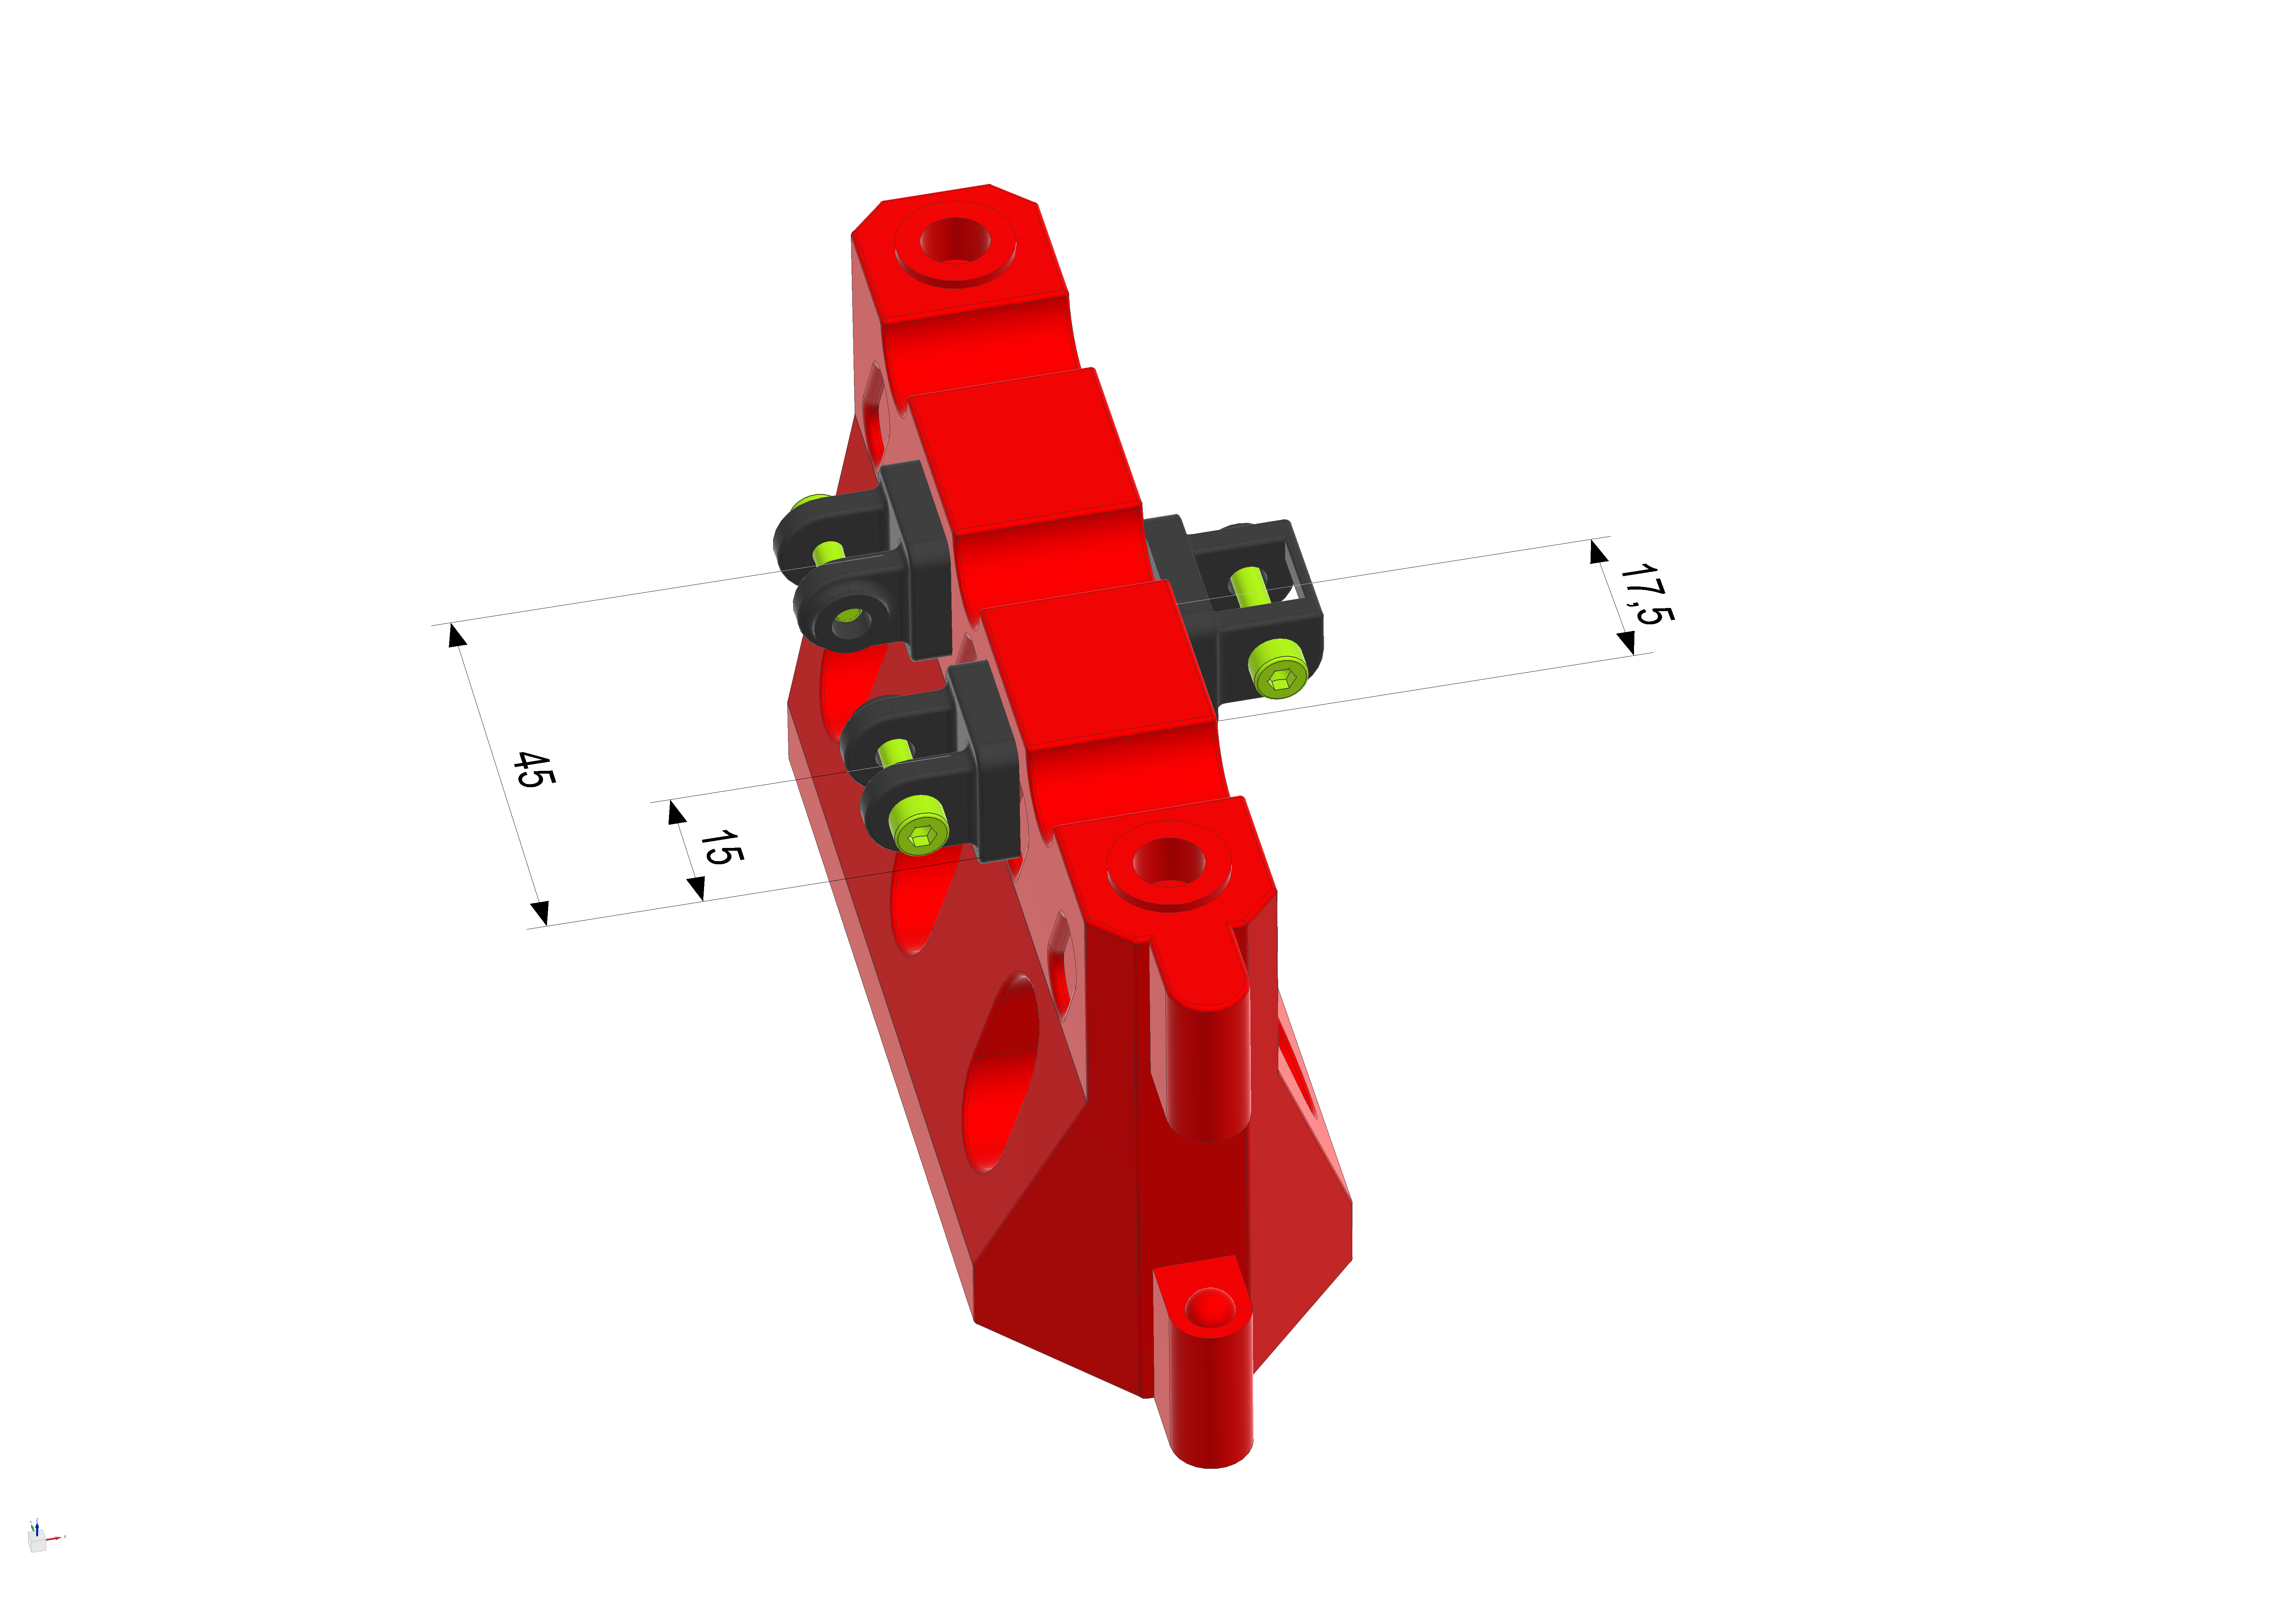
\includegraphics[width=0.95\linewidth]{assets/greifer-prototyp/Greifer_Backen_Trimetric.png} 
\caption{Position Klemmbacken}
\label{fig:obstacle_clamping_concept}
\end{figure}

Das Hindernis soll mit nur einem Motor sowohl geklemmt als auch angehoben werden. Mit einem Ultraschall-Sensor soll das vorhanden sein eines Hindernisses und die ungefähre Distanz dazu bestimmt werden. Zur genauen Bestimmung der Distanz vor dem Greifer wird ein Endschalter am Greifmechanismus verwendet.
Greifer und Endschalter werden sich an der Rückseite des Fahrzeugs befinden, der Ultraschallsensor vorne \textbf{(REF KONZEPTSKIZZE)}. somit muss sich das Fahrzeug, nach dem ein Hindernis mittels Ultraschall entdeckt wurde um 180\textdegree\ drehen, um das Hindernis anzuheben. Sobald das Hindernis angehoben ist, dreht sich das Fahrzeug wiederum um 180\textdegree\ und fährt 30mm vorwärts, um das Hindernis an dieselbe Stelle zurück zu setzen. Das Fahrzeug steht nach dem Absetzen wieder nach vorne ausgerichtet und kann geradeaus weiter fahren (siehe  Abb.\ref{fig:ablaufdiagramm-hindernis-bewegen}). 

\begin{figure}[H]
\centering
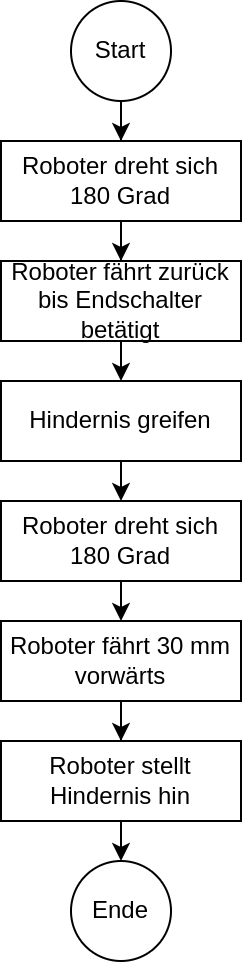
\includegraphics[width=0.2\textwidth]{assets/gesamtkonzept/ablaufdiagramm-hindernis-bewegen.png}
\caption{Ablaufdiagramm Hindernis bewegen}
\label{fig:ablaufdiagramm-hindernis-bewegen}
\end{figure}



\textbf{Skizze Ablauf Hindernis bewegen}\\
\textbf{Skizze Hindernis greifen/ absetzen}



\subsection{Schnittstellen zwischen den Kompontenten}



